\documentclass[10pt,letterpaper]{article}

\usepackage{cogsci}
\usepackage{amsmath}
\usepackage{graphicx}
\usepackage{pslatex}
\usepackage{apacite}

\graphicspath{{../figures/}}

\renewcommand{\thefootnote}{\fnsymbol{footnote}}

\makeatletter
\def\blfootnote{\xdef\@thefnmark{}\@footnotetext}
\makeatother

\title{Simultaneous unsupervised and supervised learning of
  cognitive functions \\ in biologically plausible spiking
  neural networks}

\author{{\large \bf Trevor Bekolay (tbekolay@uwaterloo.ca)} \\
  {\large \bf Carter Kolbeck (ckolbeck@uwaterloo.ca)} \\
  {\large \bf Chris Eliasmith (celiasmith@uwaterloo.ca)} \\
  Center for Theoretical Neuroscience, University of Waterloo \\
  200 University Ave., Waterloo, ON N2L 3G1 Canada}

\begin{document}

\maketitle

\begin{abstract}
  We present a novel learning rule for learning
  transformations of sophisticated neural representations
  in a biologically plausible manner.
  We show that the rule,
  which uses only information available locally
  to a synapse in a spiking network,
  can learn to transmit and bind semantic pointers.
  Semantic pointers have previously been used to build Spaun,
  which is currently the world's largest functional brain model
  \cite{Eliasmith2012}.
  Two operations commonly performed by Spaun are semantic pointer
  binding and transmission.
  It has not yet been shown
  how the binding and transmission operations can be learned.
  The learning rule combines a previously
  proposed supervised learning rule
  and a novel spiking form
  of the BCM unsupervised learning rule.
  We show that spiking BCM increases sparsity
  of connection weights
  at the cost of increased signal transmission error.
  We also demonstrate that the combined learning rule
  can learn transformations
  as well as the supervised rule and
  the offline optimization used previously.
  We also demonstrate that the combined learning rule
  is more robust to changes in parameters
  and leads to better outcomes
  in higher dimensional spaces, which is critical for
  explaining cognitive performance on diverse tasks.

  \textbf{Keywords:} synaptic plasticity; spiking neural networks;
  unsupervised learning; supervised learning;
  Semantic Pointer Architecture; Neural Engineering Framework.
\end{abstract}

In this paper, we demonstrate learning of cognitively relevant
transformations of neural representations online and in
a biologically plausible manner.
We improve upon a technique previously presented in
\citeA{MacNeil2011} by combining their error-minimization learning rule
with an unsupervised learning rule,
making it more biologically plausible and robust.\blfootnote{ \vspace{-12pt}
  \begin{description} \itemsep 0pt
    \item[BCM] Bienenstock, Cooper, Munro learning rule;
      Eq~\eqref{eq:orig-bcm}
    \item[hPES] Homeostatic Prescribed Error Sensitivity;
      Eq~\eqref{eq:hpes}
    \item[NEF] Neural Engineering Framework; see Theory
    \item[PES] Prescribed Error Sensitivity;
      Eq~\eqref{eq:pes}
    \item[SPA] Semantic Pointer Architecture; see Theory
    \item[STDP] Spike-timing dependent plasticity \cite{Bi2001}
  \end{description}
  }

There are three weaknesses with most
previous attempts at combining
supervised and unsupervised learning
in artificial neural networks
(e.g., Backpropagation [\citeNP{Rumelhart1986}],
Self-Organizing Maps [\citeNP{Kohonen1982}],
Deep Belief Networks [\citeNP{Hinton2006}]).
These approaches
1) have explicit offline training phases that are
distinct from functional use of the network,
2) require many layers with some layers
connected with supervised learning and others
with unsupervised learning, and
3) use non-spiking neuron models.
The approach proposed here overcomes these limitations.
Our approach 1) remains functional during online learning,
2) requires only two layers connected with
simultaneous supervised and unsupervised learning,
and 3) employs spiking neuron models
to reproduce central features of biological learning,
such as spike-timing dependent plasticity (STDP).

Online learning with spiking neuron models
faces significant challenges
due to the temporal dynamics of spiking neurons.
Spike rates cannot be used directly,
and must be estimated with causal filters,
producing a noisy estimate.
When the signal being estimated changes,
there is some time lag before the spiking activity
reflects the new signal,
resulting in situations during online learning
in which the inputs and desired outputs
are out of sync.
Our approach is robust to these sources of noise,
while only depending on quantities that
are locally available to a synapse.

Other techniques doing similar types of learning
in spiking neural networks
(e.g., SpikeProp [\citeNP{Bohte2002}], ReSuMe [\citeNP{Ponulak2006a}])
can learn only simple operations,
such as learning to spike at a specific time.
Others (e.g., SORN [\citeNP{Lazar2009}], reservoir computing approaches
[\citeNP{Paugam2008}]) can solve complex tasks like classification,
but it is not clear how these approaches can be applied
to a general cognitive system.
The functions learned by our approach are
complex and have already been combined into
a general cognitive system called the
Semantic Pointer Architecture (SPA).
Previously, the SPA has been used to create Spaun,
a brain model made up of 2.5 million neurons
that can do eight diverse tasks \cite{Eliasmith2012}.
Spaun accomplishes these tasks by
transmitting and manipulating semantic pointers,
which are compressed neural representations
that carry surface semantic content,
and can be decompressed to generate
deep semantic content \cite{EliasmithInPress}.
Semantic pointers are composed to represent syntactic structure
using a ``binding'' transformation,
which compresses the information in two semantic pointers
into a single semantic pointer.
Such representations can be ``collected''
using superposition, and collections
can participate in further bindings to generate deep structures.
Spaun performs these transformations by using
the Neural Engineering Framework (NEF; \citeNP{Eliasmith2003})
to directly compute static connection weights between populations.
We show that our approach can \textit{learn} to transmit, bind,
and classify semantic pointers.

\section{Theory}

\subsection{Cognitive functions with spiking neurons}

In order to characterize cognitive functions
at the level of spiking neurons,
we employ the methods of the Semantic Pointer Architecture (SPA),
which was recently used to create the world's largest
functional brain model (Spaun; \citeNP{Eliasmith2012}),
able to perform perceptual, motor, and cognitive functions.
Cognitive functions in Spaun include working memory,
reinforcement learning, syntactic generalization,
and rule induction.

The SPA is implemented using the principles of
the Neural Engineering Framework (NEF; \citeNP{Eliasmith2003}),
which defines methods to
1) \textit{represent} vectors of numbers
through the activity of populations of spiking neurons,
2) \textit{transform} those representations through
the synaptic connections between those populations, and
3) incorporate \textit{dynamics} through
connecting populations recurrently.
In the case of learning,
we exploit NEF representations in order to
learn transformations analogous
to those that can be found through the NEF's methods.

\subsubsection{Representing semantic pointers in spiking neurons}

Representation in the NEF is
similar to population coding, as proposed by
\citeA{Georgopoulos1986},
but extended to $n$-dimensional vector spaces.
Each population of neurons represents
a point in an $n$-dimensional vector space over time.
Each neuron in that population is sensitive to
a direction in the $n$-dimensional space,
which we call the neuron's \textit{encoder}.
The activity of a neuron can be expressed as
\begin{equation}
  a = G[\alpha \mathbf{e} \cdot \mathbf{x} + J_{bias}],
\end{equation}
where $G[\cdot]$ is the nonlinear neural activation function,
$\alpha$ is a scaling factor (gain) associated with the neuron,
$\mathbf{e}$ is the neuron's encoder,
$\mathbf{x}$ is the vector to be encoded, and
$J_{bias}$ is the background current of the cell.

The vector (i.e., semantic pointer)
that a population represents
can be estimated from the recent activity
of the population.
The decoded estimate, $\mathbf{\hat{x}}$,
is the sum of the activity of each neuron,
weighted by an $n$-dimensional \textit{decoder}.
\begin{equation}
  \mathbf{\hat{x}}(t) = \sum_i \mathbf{d}_i a_i(t),
\end{equation}
where $\mathbf{d}_i$ is the decoder
and $a_i$ is the activity of neuron $i$.

Neural activity is interpreted as a
filtered spike train; i.e.,
\begin{equation} \label{eq:filter-spikes}
  a_i(t) = \sum_s h(t - t_s) = \sum_s e^{-(t - t_s) / \tau_{PSC}},
\end{equation}
where $h(\cdot)$ is the exponential filter
applied to each spike,
and $s$ is the set of all spikes occurring
before the current time $t$.

The decoders are found through a least-squares minimization
of the difference between the decoded estimate
and the actual encoded vector.
\begin{equation} \label{eq:decoders}
  \mathbf{d} = \Upsilon^{-1} \Gamma \hspace{1.8em}
  \Gamma_{ij} = \int a_i a_j dx \hspace{1.8em}
  \Upsilon_j = \int a_j \mathbf{x} dx
\end{equation}

\subsubsection{Transforming semantic pointers through connection weights}

The encoders and decoders used to represent semantic pointers
also enable arbitrary transformations
(i.e., mathematical functions) of encoded semantic pointers.
If population A encodes pointer $X$,
and we want to connect it to population B, encoding pointer $Y$,
a feedforward connection with the following connection weights
transmits that semantic pointer, such that $Y \approx X$.
\begin{equation}
  \omega_{ij} = \alpha_j \mathbf{e}_j \mathbf{d}_i,
\end{equation}
where $i$ indexes the presynaptic population A,
and $j$ indexes the postsynaptic population B.
Other linear transformations
are implemented by multiplying $\mathbf{d}_i$
by a linear operator.
Nonlinear transformations are implemented
by solving for a new set of decoding weights.
This is done by minimizing the difference between
the decoded estimate of $f(\mathbf{x})$
and the actual $f(\mathbf{x})$,
rather than just $\mathbf{x}$, in Equation~\eqref{eq:decoders}.

\subsection{Supervised learning: PES rule}

\citeA{MacNeil2011} proposed a learning rule
that minimizes the error minimized
in Equation~\eqref{eq:decoders} online.
\begin{align} \label{eq:pes}
  \Delta \mathbf{d}_i &= \kappa \mathbf{E} a_i \nonumber \\
  \Delta \omega_{ij} &= \kappa \alpha_j \mathbf{e}_j \cdot \mathbf{E} a_i,
\end{align}
where $\kappa$ is a scalar learning rate,
$\mathbf{E}$ is a vector representing the error we wish to minimize,
and other terms are as before.

When put in terms of connections weights ($\omega_{ij}$),
the rule resembles backpropagation.
The quantity $\alpha_j \mathbf{e}_j \cdot \mathbf{E}$
is analogous to the local error term
$\delta$ in backpropagation \cite{Rumelhart1986};
they are both a means of translating a global error signal
to a local error signal that can be used to
change an individual synaptic connection weight.
The key difference between this rule
and backpropagation is that the global-to-local mapping
is done by imposing the portion of the error vector space
each neuron is sensitive to via its encoder.
This limits flexibility, but removes the dependency
on global information, making the rule biologically plausible.
We will refer to Equation~\eqref{eq:pes} as
the Prescribed Error Sensitivity (PES) rule.

\subsection{Unsupervised learning: Spiking BCM rule}

A Hebbian learning rule widely studied
in the context of the vision system
is the BCM rule \cite{Bienenstock1982}.
This rule has been used to explain orientation selectivity
and ocular dominance \cite{Bienenstock1982}.
Theoretically, it has been asserted that BCM is equivalent
to triplet-based STDP learning rules \cite{Pfister2006}.

The general form is
\begin{equation} \label{eq:orig-bcm}
  \Delta \omega_{ij} = a_i a_j (a_j - \theta),
\end{equation}
where $\theta$ is the \textit{modification threshold}.
When the postsynaptic activity, $a_j$, is
greater than the modification threshold,
the synapse will be potentiated;
when the postsynaptic activity is less than the modification threshold,
the synapse will be depressed.

The modification threshold reflects the expectation
of a cell's activity.
It is typically calculated as
the temporal average of the cell's activity
over a long time window (on the order of hours).
The intuition behind BCM is that cells
driven above their expectation
must be playing an important role in a circuit,
so their afferent synapses become potentiated.
Cells driven less than normal have synapses depressed.
If either of these effects persists long enough,
the modification threshold changes
to reflect the new expectation
of the cell's activity.

However, BCM as originally formulated
is based on non-spiking rate neurons.
We implement BCM in biologically plausible spiking networks
by interpreting neural activity as
spikes that are filtered by
a postsynaptic current curve.
\begin{align} \label{eq:bcm}
  \Delta \omega_{ij} &= \kappa \alpha_j a_i a_j (a_j - \theta) \nonumber \\
  \theta(t) &= e^{-t / \tau} \, \theta(t-1) +
               (1 - e^{-t / \tau} \, a_j(t)),
\end{align}
where $a$, the activity of a neuron,
is interpreted as a filtered spike train,
as in Equation~\eqref{eq:filter-spikes},
and $\tau$ is
the time constant of
the modification threshold's exponential filter.

With our spiking BCM implementation,
we aim to test the claim that BCM is equivalent
to triplet STDP rules.
Functionally, we hypothesize that
unsupervised learning
will have a small detrimental effect
on the function being computed by a weight matrix,
but will result in weight sparsification.

\subsection{Simultaneous supervised and unsupervised learning: hPES rule}

The PES rule gives us the ability to
minimize some provided error signal,
allowing a network to
learn to compute a transformation online.
However, biological synapses can change
when no error signal is present.
More practically,
transformation learning may be easier
in more sparse systems.
For these reasons, we propose a new learning rule
that combines the error-minimization abilities of the PES rule
with the biological plausibility and sparsification
of the spiking BCM rule.
The rule is a weighted sum of the
terms in each rule.
\begin{equation} \label{eq:hpes}
  \Delta \omega_{ij} = \kappa \, \alpha_j a_i \left(
    S \, \mathbf{e}_j \cdot \mathbf{E} + (1 - S) \, a_j(a_j - \theta) \right),
\end{equation}
where $0 \le S \le 1$ is the relative weighting of
the supervised term over the unsupervised term.
Note that this rule is a generalization
of the previously discussed rules;
if we set $S = 1$,
this rule is equivalent to PES, and
if we set $S = 0$,
this rule is equivalent to spiking BCM.

We hypothesize that the unsupervised
component helps maintain homeostasis
while following the error gradient defined
by the supervised component.
Because of this, we call the rule
the homeostatic Prescribed Error Sensitivity (hPES) rule.
We hypothesize that this rule will
be able to learn the same class
of transformations that the PES rule can learn,
and that this class includes operations
critical to cognitive representation,
such as semantic pointer binding.

Note that a similar combination can be done
with other supervised learning rules that
modify connection weights.
A more general form of Equation~\eqref{eq:hpes}
would replace the local error quantity
$\mathbf{e}_j \cdot \mathbf{E}$ with $\delta$,
which could be determined through any method.
However, for clarity, we will use hPES
to refer to the specific form in
Equation~\eqref{eq:hpes}.

\section{Methods}

We performed three experiments in order to
test our hypotheses about the hPES rule.
Experiments were implemented in the Nengo
simulation environment, in which we implemented
the PES, spiking BCM, and hPES learning rules.
All experiments use leaky integrate-and-fire
neurons with default parameters.
The scripts used to implement
and analyze these experiments
are MIT licensed and available at
\url{http://github.com/tbekolay/cogsci2013}.

\subsubsection{Experiment 1: Unsupervised learning}

We constructed a network composed of two populations
connected in a feedforward manner
such that one population provides input to the other.
The network can be run in a ``control'' regime,
in which the weights between the two populations
are solved for with the NEF's least-squares optimization
and do not change, or in a ``learning'' regime,
in which the weights are the same as the control network,
but change over time according to the hPES rule \eqref{eq:hpes}
with $S = 0$ (i.e., according to the spiking BCM rule [\ref{eq:bcm}]).
This experiment tests the hypothesis that the unsupervised
component of the hPES rule increases sparsity
of the connection weight matrix.

\subsubsection{Experiment 2: Supervised learning}

We constructed a network composed of two populations
connected in a feedforward manner,
and one population that provides
an error signal to the downstream population.
The network can be run in a ``control'' regime,
in which the weights between the two populations
are computed to transmit a three-dimensional semantic pointer,
or to bind two three-dimensional semantic pointers
into one three-dimensional pointer.
The network can be run in a ``learning'' regime,
in which the weights between the two populations
are initially random
and are modified over time by the hPES rule.
This experiment tests the hypothesis that the hPES
rule can learn to transmit and bind semantic pointers
as well as the control network and the supervised
learning rule (i.e., hPES with $S=1$).

\subsubsection{Experiment 3: Digit classification}

In order to investigate how
simultaneous supervised and unsupervised learning
scales in higher dimensional situations,
we constructed a network similar to that in Experiment 2,
but whose input is handwritten digits.\footnote{Digits
  from MNIST: \url{http://yann.lecun.com/exdb/mnist/}}
In order to be computationally tractable,
the 28-by-28 pixel images were compressed to a 50-dimensional
semantic pointer using a sparse deep belief network
that consists of four feedforward
Restricted Boltzmann Machines
trained with a form of contrastive divergence
(full details in \citeNP{Tang2010}).
Those 50-dimensional pointers were projected to
an output population of 10 dimensions,
where each dimension represents
the confidence that the input representation should
be classified into one of the 10 possible digits.
The classified digit is the one corresponding
to the dimension with the highest activity
over 30 ms when a 50-dimensional input is presented.
60,000 labeled training examples
were shown to the network while
the hPES rule was active.
The network was then tested with 10,000
training examples in which the label
was not provided.
The results are compared to an analogous control network,
in which the 50-dimensional pointers are classified
with a cleanup memory whose connection weights
are static, as in \citeA{Eliasmith2012}.
This experiment examines how well the hPES rule scales
to high-dimensional spaces.

\subsubsection{Learning parameters}

While there are many hundreds of parameters
involved in each network simulation,
the vast majority are randomly selected
within a biologically plausible range
without significantly affecting performance.
Some parameters, especially those affecting
the learning rule, can have a significant performance effect.
These significant parameters and the values
used in specific simulations are listed
in Tables~\ref{tab:params-1} and \ref{tab:params-2}.
These parameters were optimized
with a tree of Parzens estimators approach,
using the \texttt{hyperopt} package \cite{Bergstra2013}.

\begin{table}[!ht]
\begin{center} 
\caption{Parameters used for transmitting semantic pointers}
\vspace{0.2ex}
\label{tab:params-1} 
\begin{tabular}{llcc} 
\hline
Parameter & Description & Value \\
\hline
$N / D$ & Neurons per dimension & 25 \\
$\kappa$ & Learning rate & $3.51 \times 10^{-3}$ \\
$S$ & Supervision ratio & 0.798 \\
$\kappa$ for $S = 1$ & Learning rate (PES) & $2.03 \times 10^{-3}$\\ 
\hline
\end{tabular} 
\end{center}
\begin{center} 
\caption{Parameters used for binding and classifying SPs}
\vspace{0.2ex}
\label{tab:params-2} 
\begin{tabular}{llcc} 
\hline
Parameter & Description & Value \\
\hline
$N / D$ & Neurons per dimension & 25 \\
$\kappa$ & Learning rate & $2.38 \times 10^{-3}$ \\
$S$ & Supervision ratio & 0.725 \\
$\kappa$ for $S = 1$ & Learning rate (PES) & $1.46 \times 10^{-3}$ \\ 
\hline
\end{tabular} 
\end{center}
\end{table}

\section{Results}

\subsection{hPES replicates STDP results}

Previously, \citeA{Pfister2006}
have theorized that BCM and STDP are equivalent.
Our experiments support this theory.
Varying the amount of time between presynaptic
and postsynaptic spikes results in an STDP curve
extremely similar to the classical
\citeA{Bi2001} STDP curve
(Figure~\ref{fig:stdp-curve}).

\begin{figure}[ht]
\begin{center}
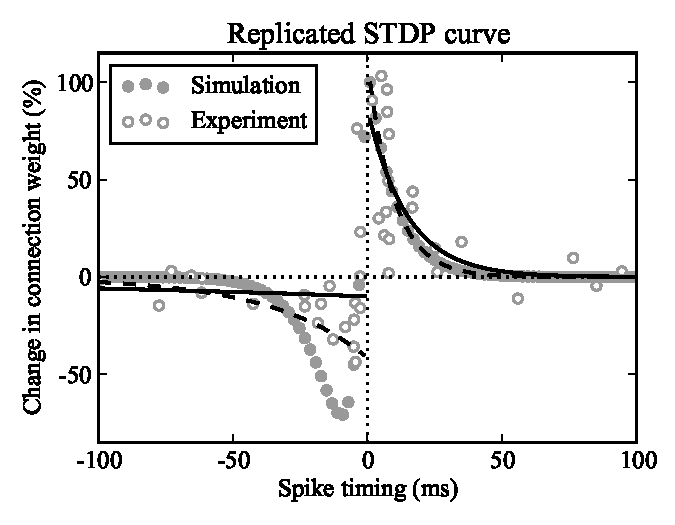
\includegraphics[width=\columnwidth]{fig1-bcm-stdp}
\end{center}
\caption{STDP curve replicated by two neurons
  connected with the hPES rule, $S = 0$.
  Solid and dashed lines are best fits of the curve
  $a\,e^{-x / \tau}$ for the experimental
  and simulated data, respectively.
  Experimental data from \citeA{Bi2001}.}
\label{fig:stdp-curve}
\end{figure}

However, these STDP curves do not capture
the frequency dependence of STDP.
In order to capture those effects,
modellers have created STDP rules that take into
account triplets and quadruplets of spikes,
rather than just pre-post spike pairings \cite{Pfister2006}.
These rules are able to replicate
the frequency dependence of the STDP protocol.
Figure~\ref{fig:stdp-freq} shows that,
despite being a much simpler rule,
the hPES rule with $S = 0$
also exhibits frequency dependence.

\begin{figure}[ht]
\begin{center}
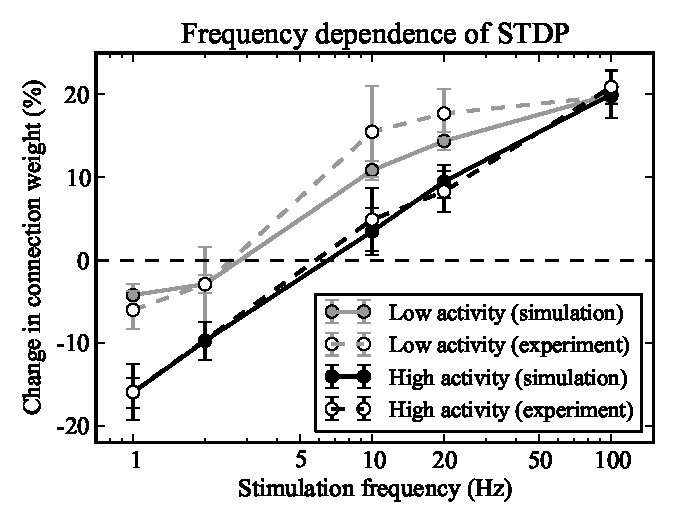
\includegraphics[width=\columnwidth]{fig2-bcm-stdp-frequency}
\end{center}
\caption{STDP frequency dependence replicated by two neurons
  connected with the hPES rule, $S = 0$.
  This also demonstrates the effect of different $\theta$
  values on the frequency dependence curve.
  Experimental data from \citeA{Kirkwood1996}.}
\label{fig:stdp-freq}
\end{figure}

\subsection{hPES encourages sparsity while increasing signal
  transmission error}

When the hPES rule is applied to
a network that has been optimized
to implement semantic pointer transmission,
the hPES rule with no supervision ($S = 0$)
increases signal transmission error at
a rate proportional to the learning rate.
Figure~\ref{fig:bcm} (top) shows the gradual
decrease in accuracy over 200 seconds of simulation
with an artificially large learning rate.
Figure~\ref{fig:bcm} (bottom) shows that the sparsity
of the weight matrix, as measured by the Gini index,
increases over time.
Therefore, the hPES rule with $S = 0$
increases network sparsity
at the cost of an increase in signal transmission error.

\begin{figure}[ht]
\begin{center}
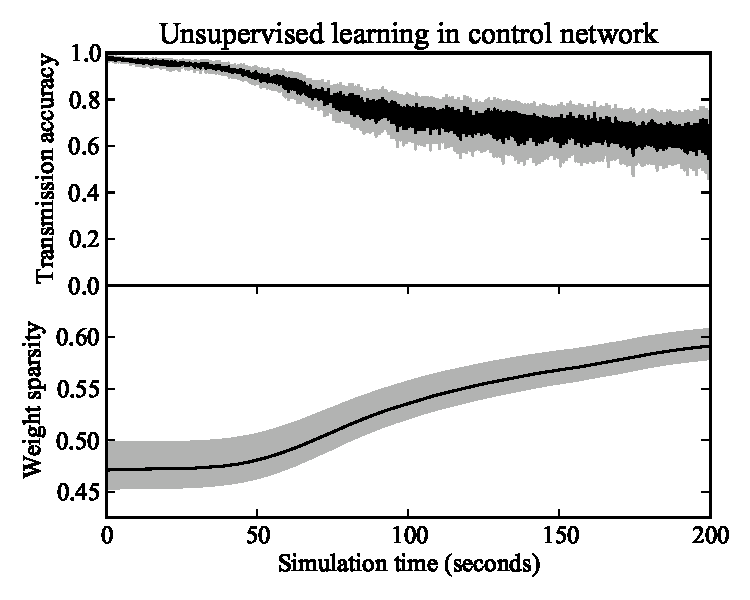
\includegraphics[width=\columnwidth]{fig3-bcm}
\end{center}
\caption{Data gathered from 50 trials of Experiment 1;
  filled region represents a bootstrapped 95\% confidence interval.
  (Top) Accuracy of signal transmission.
  Accuracy is proportional to negative mean squared error,
  scaled such that accuracy of 1.0
  denotes a signal identical to that transmitted by the
  NEF optimal weights with no learning, and
  accuracy of 0.0 represents no signal transmission
  (i.e., the error is equal to the signal).
  (Bottom) Sparsity of the connection weight matrix over time,
  as measured by the Gini index. This demonstrates
  the expected tradeoff between sparsity and accuracy.}
\label{fig:bcm}
\end{figure}

\subsection{hPES can learn cognitive functions}

The error in the learned networks
relative to the mean of 10 control networks
can be seen decreasing over time in Figure~\ref{fig:learn}.
The parameters used for Figure~\ref{fig:learn}
are listed in Tables~\ref{tab:params-1} and \ref{tab:params-2}.
The transformations are learned quickly
(approximately 25 seconds for transmission, 45 seconds for binding).
Therefore, the central binding and transmission
operations of the SPA
are learnable with the hPES rule.

Critically, while hPES without error sensitivity
introduces error while increasing sparsity
(see Figure~\ref{fig:bcm}), with error sensitivity,
this error can be overcome.
Interestingly, binding,
the intuitively more complex operation,
is more reliably learned than transmission.
This is due to how effectively
the NEF can optimize weights to perform
linear transformations like transmission
in the control networks.

\begin{figure}[ht]
\begin{center}
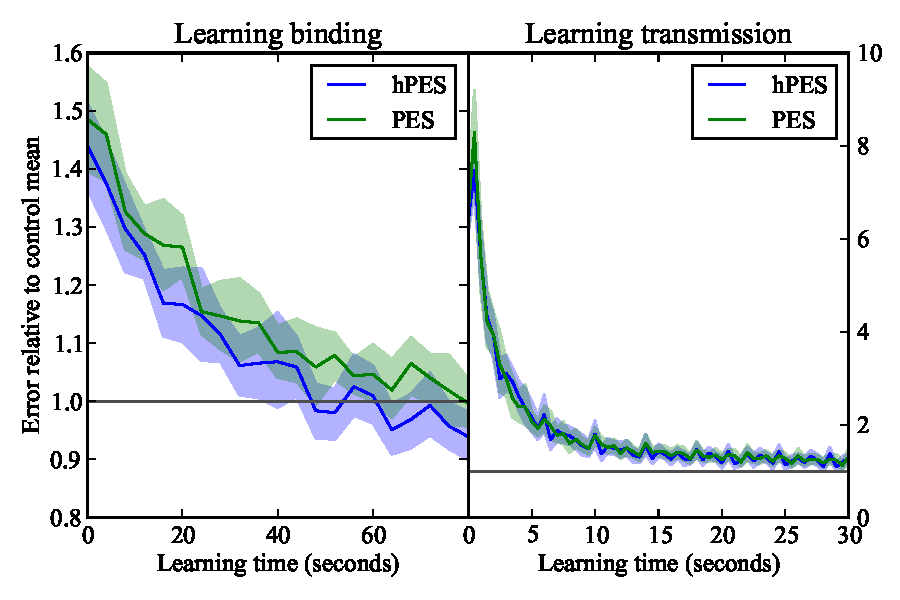
\includegraphics[width=\columnwidth]{fig4-learn-curves}
\end{center}
\caption{Error of learning networks over time compared
  to the mean error of 10 control networks.
  Each type of network is generated and simulated 15 times.
  For the binding network, every 4 seconds,
  the learning rule is disabled and error is accumulated
  over 5 seconds.
  For the transmission network, every 0.5 seconds,
  the learning rule is disabled,
  and error is accumulated over 2 seconds.
  Filled regions are bootstrapped 95\% confidence intervals.
  Time is simulated time, not computation time.}
\label{fig:learn}
\end{figure}

As a proof of concept that the hPES rule
scales to high-dimensional spaces,
Table~\ref{tab:digits} shows that 
the learned handwritten digit classification network
classifies digits more accurately than Spaun's cleanup memory
\cite{Eliasmith2012}.
This supports the suggestion that the hPES rule
scales to high-dimensional spaces.
While the hPES rule with $S < 1$
achieved higher classification accuracy
than hPES with $S = 1$,
not enough trials were attempted to
statistically confirm a benefit to combined
unsupervised and supervised learning for classifying
handwritten digits.

\begin{table}[!ht]
\begin{center} 
\caption{Classification accuracy of handwritten digits} 
\label{tab:digits} 
\vskip 0.12in
\begin{tabular}{ll} 
\hline
Classification technique & Accuracy \\
\hline
Cleanup memory (Spaun)   & 94\% \\
hPES learning, $S = 1$   & 96.31\% \\
hPES learning            & 98.47\% \\
\hline
\end{tabular} 
\end{center} 
\end{table}

\subsection{hPES is less sensitive to parameters}

The parameters of the hPES rule were optimized with
$S$ fixed at 1 for 50 simulations of binding and transmission.
A separate parameter optimization that allowed $S$ to change
was done for 50 simulations of binding and transmission.

\begin{figure}[ht]
\begin{center}
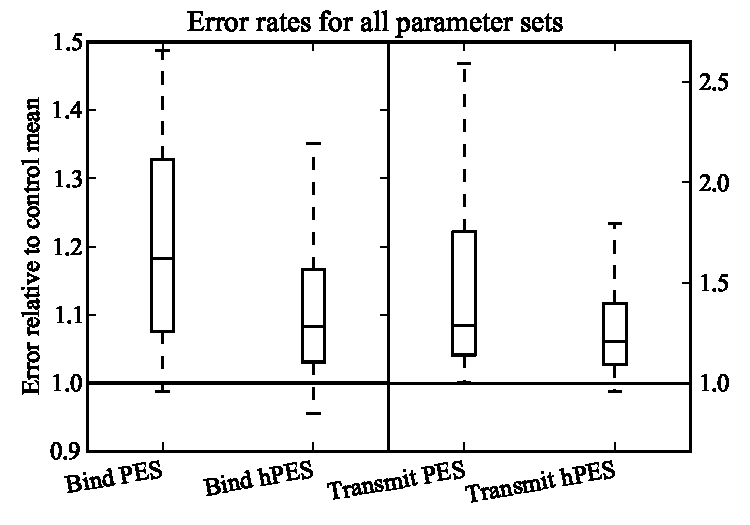
\includegraphics[width=\columnwidth]{fig5-param-boxplot}
\end{center}
\caption{Summary of error rates for networks used
  to optimize learning parameters. Each column
  summarizes 50 experiments of the labeled condition.
  Boxes indicate the median and inter-quartile range,
  and whiskers indicate the inner fence (i.e.,
  $Q_1 - 1.5 \: IQR$ and $Q_3 + 1.5 \: IQR$).
  Outliers are not shown.}
\label{fig:params}
\end{figure}

Surprisingly, despite optimizing over an additional dimension,
when $S$ was allowed to change, error rates were
lower during the optimization process
for the binding network but not the transmission network.
In both cases, the interquartile range of the hPES rule's
performance when $S$ was allowed to change is lower.
Figure~\ref{fig:params} summarizes the performance of
all 200 networks generated for parameter optimization.
While in all four cases parameters were found that achieve
error rates close to the control networks,
hPES was more robust to changes
in parameters when $S$ was allowed to change.
This suggests that unsupervised learning
may be beneficial in high-dimensional nonlinear situations.

\section{Discussion}

In this paper, we have presented a novel learning rule
for learning cognitively relevant transformations
of neural representations
in a biologically plausible manner.
We have shown that the unsupervised component of the rule
increases sparsity of connection weights
at the cost of increased signal transmission error.
We have also shown that the combined learning rule, hPES,
can learn transformations as well as the supervised rule
and the offline optimization done in the Neural Engineering Framework.
We have demonstrated that the combined learning rule
is more robust to changes in parameters
when learning nonlinear transformations.

However, it is still the case that
the parameters of the learning rule
were optimized for each transformation learned.
This is a challenge shared by all learning rules,
but in the context of biologically plausible simulations,
there is the additional question of
the biological correlate of these parameters.
It could be the case that these parameters
are a result of the structure of the neuron,
and therefore act as a fixed property of the neuron.
However, it could also be the case that
these parameters are related to the activity of the network,
and are modified by each neuron's activity,
or by the activity of some external
performance monitoring signal.
Examining these possibilities is the subject
of future work.

\section{Acknowledgments}

This work was supported by the Natural Sciences
and Engineering Research Council of Canada,
Canada Research Chairs,
the Canadian Foundation for Innovation
and the Ontario Innovation Trust.
We also thank James Bergstra for creating
the \texttt{hyperopt} tool and assisting
with its use.

\bibliographystyle{apacite}

\setlength{\bibleftmargin}{.125in}
\setlength{\bibindent}{-\bibleftmargin}

\bibliography{bekolay}

\end{document}
